\subsection{Repartition Frequency}
The results of our repartition frequency experiments are shown in Figure \ref{fig:FrequencySensitivity}. We ran experiments using 8 partitions based on results from the partition count results, discussed in the Partition Count section. The experiments were run using 42,875 blocks on a single machine with 12 and 16 cores. The repartition frequency determines how often the RDD gets redistributed among the executor nodes to maintain load balance. As can be seen in the results, repartitioning more often generally leads to faster runs with a repartion period on the order ~15 discontinuities giving close to optimal performance. \par

There is a significant spike in the time it took the runs to complete when using a repartition period of 50 joints. This can be explained when considering the number of joints in the data set was 105 - the RDD was repartitioned twice during the computations and the last repartition occured when the calculations were almost completed and the RDD was close to its maximum size. Clearly, this is not a good time to repartition since the amount of data that has to be shuffled is close to the maximum value and the gains from load balancing will be short lived as the computations are nearly completed. \par

\begin{figure}
  \centering
  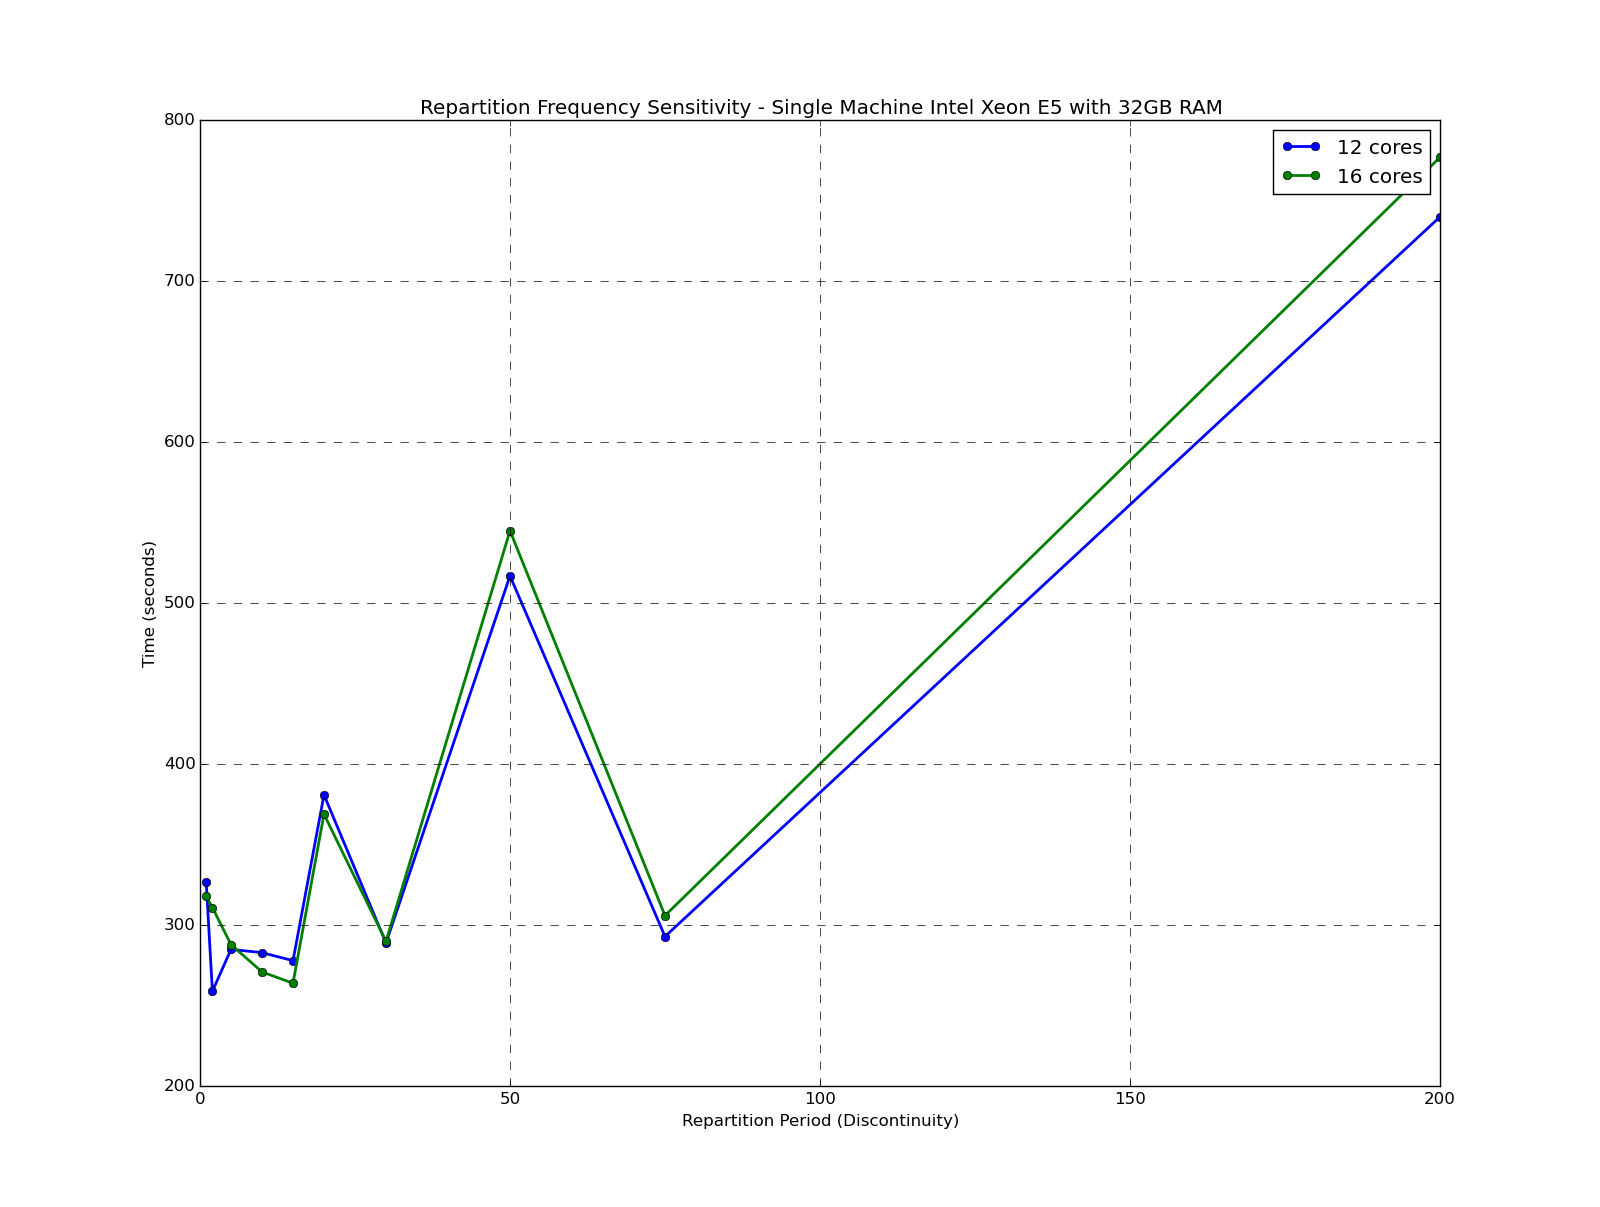
\includegraphics[width=0.4\textwidth]{FrequencySensitivity} 
  \label{fig:FrequencySensitivity}           
\end{figure}

Conversely, computation times close to optimal were achieved by repartitioning only once after 75 joints had been processed. This makes intuitive sense as it seems to strike a balance between minimizing shuffling  while  maintaining a balanced load. It is possible that as a ``rule of thumb'' repartitioning only once when approximately 75\% of the joints have been proccessed will give timings close enough to optimum for general use. Unfortunately, there was insufficient time to investigate this phenomenon further due to time constraints. \par

Lastly, the increased computation times at large repartition periods illustrate how load imbalance significantly deteriorates the efficiency of the computations. For our experiments, a repartition period of 200 implies that the RDD was not repartitioned at all since only 105 joints were processed. As previously discussed, this caused tremendous load-imbalance due to the nature of the input data set. \par

\subsection{Partition Count}
Figure \ref{fig:PartCount} shows the results of our sensitivity analysis for RDD partitioning. Tests were run using a repartition period of 15 joints - the results of the repartition frequency experiments indicated that this would be close to optimum for ~42,000 blocks. The results for number of partitions are somewhat counter intuitive - in both cases the best speeds were achieved by having less partitions than the number of cores. \cite{sparkTuning} recommends having more partitions than the number of cores as general rule to increase parallelism; however, this does not appear to be the case for our analysis. It is possible that in our case the tasks that need to be completed on each RDD are more time consuming since the cutting and intersection methods invoke a linear program solver for each joint that is processed. This could lead to long idle times for threads that end up taking a lot of memory and computational capacity away from the actual computations. More experimentation and a deeper understanding of how Spark manages RDD's and parallism is necessary to fully understand this behavior. \par

\begin{figure}
  \centering
  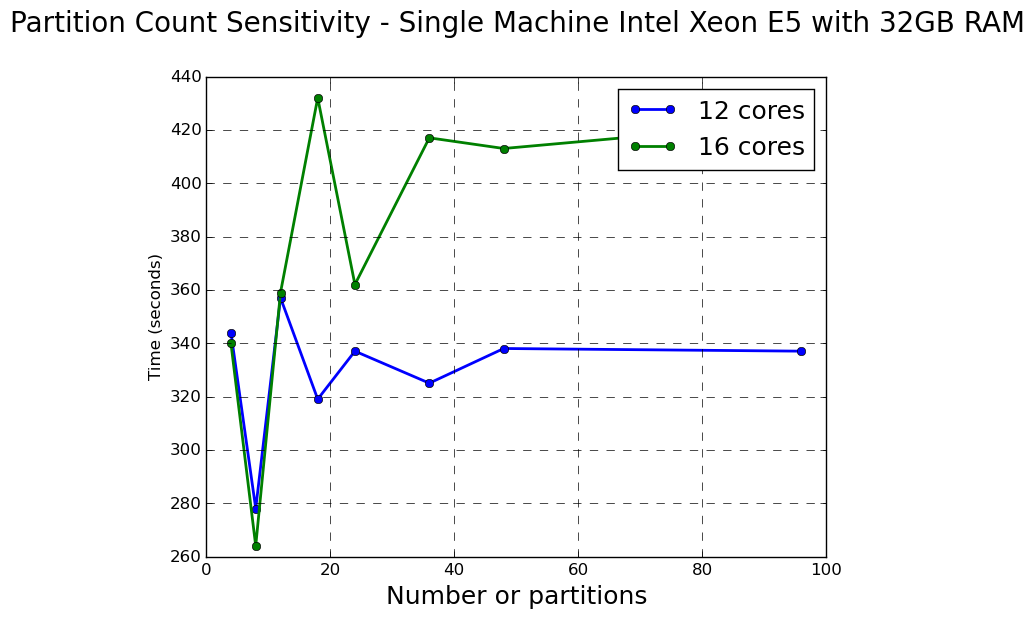
\includegraphics[width=0.4\textwidth]{PartCount} 
  \label{fig:PartCount}           
\end{figure}

What is clear from the experiments though is that getting the partition number wrong actually leads to worse performance when using more cores. Only by selecting the correct amount of partitions does it lead to increased performance for more computing power - 16 cores only outperformed 12 cores when using 8 partitions. For all other partition values tested 12 cores are faster than 16, especially when using more partitions.

\subsection{Weak Scaling}

\subsection{Strong Scaling}
